\chapter{Parallélisation Kokkos et portabilité GPU}
\label{chap:kokkos}

Le sujet propose Kokkos comme alternative à OpenMP. Nous l'avons implémenté à la fois pour répondre à cette option et pour explorer la \textbf{portabilité GPU} : avec Kokkos, le même code source compile pour OpenMP, CUDA, HIP, ou SYCL selon le backend choisi à la compilation.

\section{Pourquoi Kokkos ?}

\subsection{Le problème de la portabilité GPU}

Sans Kokkos, porter WFC sur GPU exigerait :
\begin{itemize}
    \item Une réécriture en CUDA (ou HIP, ou SYCL) avec gestion explicite de la mémoire host/device.
    \item Le maintien de \textbf{deux} bases de code séparées (CPU + GPU).
    \item L'apprentissage d'un dialecte par vendor (NVIDIA / AMD / Intel).
\end{itemize}

Kokkos abstrait ces différences. Le développeur écrit un \textbf{kernel parallèle} (\texttt{parallel\_for}) avec des \textbf{vues} (\texttt{View<T*>}) ; le compilateur Kokkos génère le code adapté au backend cible.

\subsection{Tradeoffs}

\begin{itemize}
    \item \textbf{Avantage} : un seul code source qui tourne sur CPU, GPU NVIDIA, GPU AMD.
    \item \textbf{Inconvénient} : conventions à respecter (\texttt{KOKKOS\_INLINE\_FUNCTION}, pas d'allocation dynamique dans les kernels, capture par valeur).
    \item \textbf{Inconvénient} : le code peut sembler verbeux comparé à du CUDA pur.
\end{itemize}

\section{Architecture du backend Kokkos}

\subsection{Vue d'ensemble}

\begin{figure}[H]
\centering
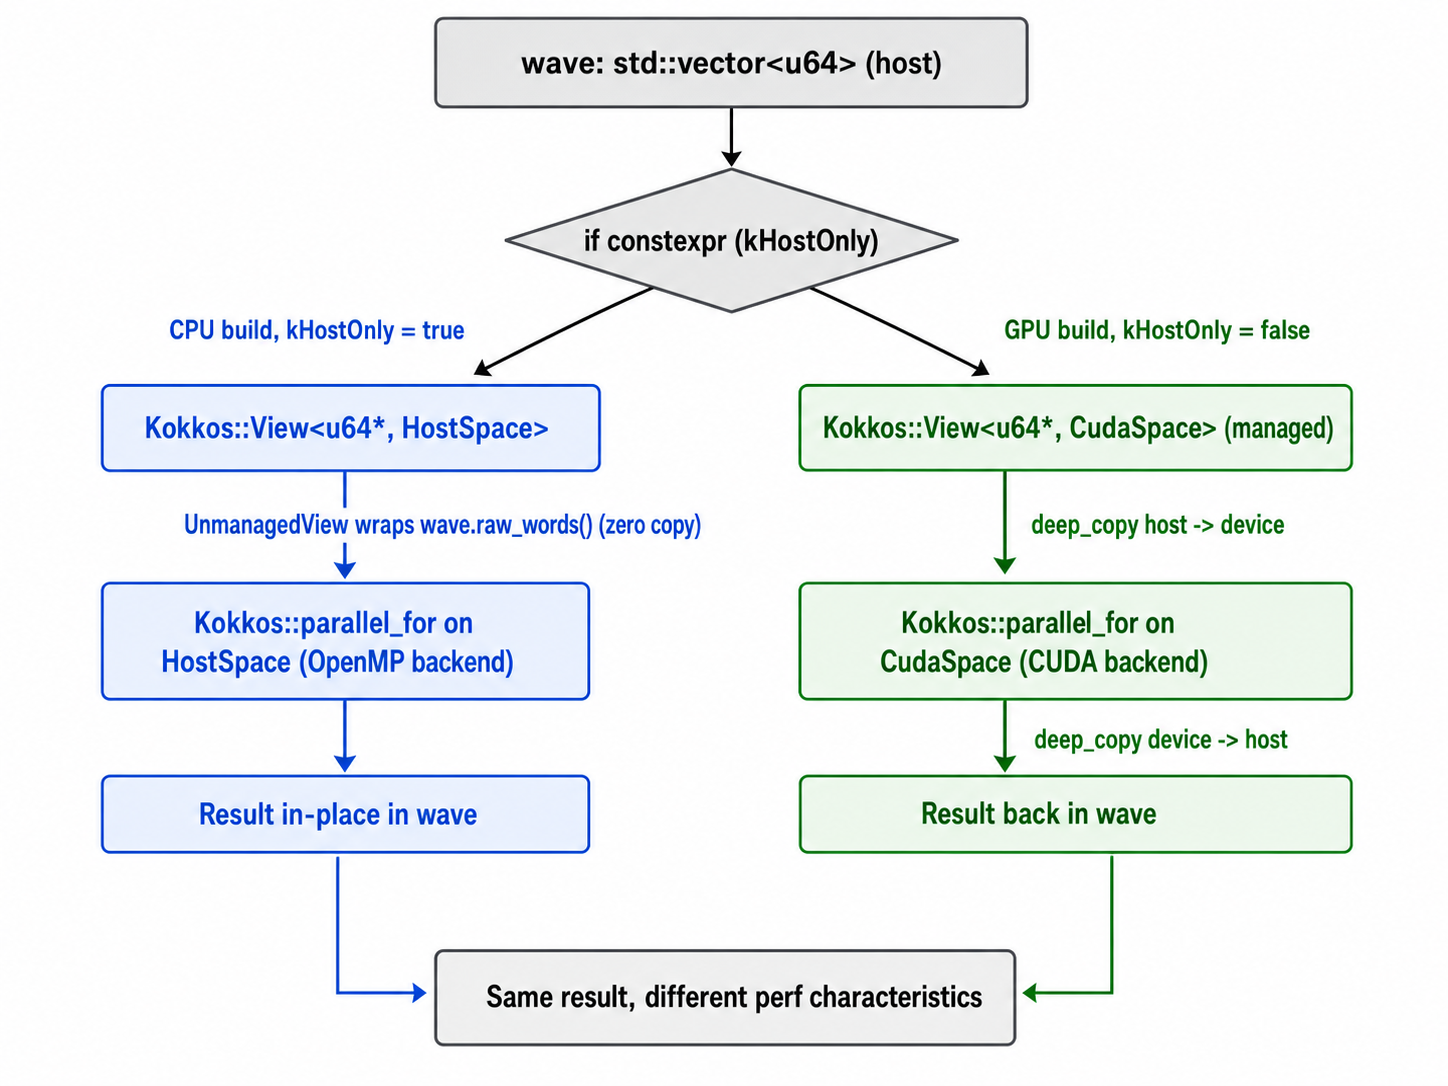
\includegraphics[width=0.85\linewidth]{results/figures/schemas/kokkos_architecture.png}
\caption{Architecture Kokkos pour la propagation BFS, avec branche \texttt{kHostOnly} compile-time choisissant zero-copy ou deep\_copy.}
\label{fig:kokkos_architecture}
\end{figure}

Le backend Kokkos repose sur trois composants :

\begin{enumerate}
    \item \textbf{Vues GPU-accessibles} (\texttt{Kokkos::View<u64*, MemSpace>}) pour la wave et les règles d'adjacence.
    \item \textbf{Fonctor de propagation} (\texttt{PropagateOp}) marqué \texttt{KOKKOS\_INLINE\_FUNCTION}, dispatché par \texttt{Kokkos::parallel\_for}.
    \item \textbf{Branche \texttt{kHostOnly} compile-time} qui choisit zero-copy (CPU build) ou \texttt{deep\_copy} (GPU build).
\end{enumerate}

\subsection{Détection compile-time du backend}

\begin{lstlisting}[language=C++]
using ExecSpace = Kokkos::DefaultExecutionSpace;
using MemSpace = ExecSpace::memory_space;

// True quand le memory space par défaut est HostSpace (build CPU OpenMP).
// False sur build CUDA / HIP (memory space sur device).
constexpr bool kHostOnly = std::is_same<MemSpace, Kokkos::HostSpace>::value;
\end{lstlisting}

Cette constexpr permet ensuite de choisir entre zero-copy et deep\_copy via \texttt{if constexpr} :

\begin{lstlisting}[language=C++]
if constexpr (kHostOnly) {
    // Wrap directement le buffer host de Wave (zero-copy)
    s.wave_view = U64View(wave.raw_words(), wave.total_words());
} else {
    // Buffer device séparé, deep_copy host -> device
    s.wave_view = U64View("wfc_wave", wave.total_words());
    Kokkos::deep_copy(s.wave_view, host_wave_view);
}
\end{lstlisting}

\textbf{Conséquence} : le build CPU paie zéro overhead (le compilateur évalue \texttt{kHostOnly = true} et inline directement). Le build GPU paie la copie host↔device, mais c'est inévitable sur cette architecture.

% =============================================================================
\section{Stack arrays plutôt que heap dans le kernel}
\label{sec:kokkos:stack_arrays}
% =============================================================================

\begin{important}{Contrainte GPU : pas de heap dans le kernel}
Sur device, l'allocation dynamique (\texttt{new}, \texttt{std::vector::resize}) est soit interdite, soit catastrophique en perf. Le code GPU doit utiliser uniquement des stack arrays de taille connue à la compilation.
\end{important}

Notre solution : \texttt{constexpr std::size\_t MAX\_WORDS\_PER\_CELL = 8} (couvre jusqu'à 512 tuiles, largement suffisant pour nos samples).

\begin{lstlisting}[language=C++, caption={PropagateOp fonctor avec stack arrays}]
struct PropagateOp {
    WaveView_K wave;
    RulesView_K rules;
    IntView frontier;
    IntView next_frontier;
    IntView next_count;
    U8View in_queue;
    IntView contradiction_flag;

    KOKKOS_INLINE_FUNCTION
    void operator()(const int idx) const {
        if (Kokkos::atomic_load(&contradiction_flag(0))) return;

        const int c = frontier(idx);
        const int W = wave.words_per_cell;

        // Stack snapshot anti-race (1 mot pour L<=64, jusqu'a 8)
        std::uint64_t snap[MAX_WORDS_PER_CELL];
        for (int w = 0; w < W; ++w) snap[w] = wave.words(c * W + w);

        for (int dy = ...; ...) for (int dx = ...; ...) {
            const int nc = wave.torus_idx(...);

            // Stack accumulator
            std::uint64_t allowed[MAX_WORDS_PER_CELL];
            for (int w = 0; w < W; ++w) allowed[w] = 0ULL;
            // ... union over snap's set bits ...

            bool changed = false;
            for (int i = 0; i < W; ++i) {
                const u64 mask = allowed[i];
                if (mask == 0xFFFFFFFFFFFFFFFFULL) continue;
                // Relaxed-load skip (mirror OMP optim)
                const u64 cur = Kokkos::atomic_load(&wave.words(nc * W + i));
                if ((cur & ~mask) == 0ULL) continue;
                const u64 old_val = Kokkos::atomic_fetch_and(
                    &wave.words(nc * W + i), mask);
                if ((old_val & ~mask) != 0ULL) changed = true;
            }
            if (changed) { /* CAS dedup, push to next_frontier */ }
        }
    }
};
\end{lstlisting}

% =============================================================================
\section{Optimisations OMP propagées au kernel Kokkos}
\label{sec:kokkos:propagated}
% =============================================================================

Toutes les optimisations validées en OMP ont été propagées au kernel Kokkos :

\begin{table}[H]
\centering
\begin{tabularx}{\textwidth}{lX}
\toprule
\textbf{Optim OMP} & \textbf{Implémentation Kokkos} \\
\midrule
Snapshot anti-race & Stack array \texttt{snap[MAX\_WORDS\_PER\_CELL]} \\
\midrule
Mask all-ones skip & \texttt{if (mask == \textasciitilde{}0ULL) continue;} avant atomic \\
\midrule
Relaxed-load skip avant atomic & \texttt{Kokkos::atomic\_load} puis \texttt{Kokkos::atomic\_fetch\_and} \\
\midrule
CAS dedup sur in\_queue & \texttt{Kokkos::atomic\_compare\_exchange} \\
\midrule
Counter atomique \texttt{next\_frontier} & \texttt{atomic\_fetch\_add(\&next\_count(0), 1)} \\
\bottomrule
\end{tabularx}
\caption{Optimisations OMP transposées au backend Kokkos. Le code device respecte les mêmes invariants algorithmiques.}
\label{tab:kokkos:optims}
\end{table}

% =============================================================================
\section{Cleanup correct : \texttt{push\_finalize\_hook}}
\label{sec:kokkos:cleanup}
% =============================================================================

\begin{important}{Bug subtil rencontré : View deallocated after Kokkos::finalize}
Un solver Kokkos cache des Views dans des variables \texttt{static thread\_local} (rules cache, scratch buffers). À process exit, l'ordre de destruction est : \texttt{Kokkos::finalize()} → variables \texttt{thread\_local}. Le second tente de désallouer des buffers Kokkos après que le memory subsystem a été tear-down. Erreur runtime.
\end{important}

\subsection{Solution : \texttt{push\_finalize\_hook}}

Kokkos fournit \texttt{push\_finalize\_hook} qui enregistre une callback exécutée \textit{pendant} \texttt{Kokkos::finalize}, avant le tear-down.

\begin{lstlisting}[language=C++]
void install_finalize_hook_once() {
    static thread_local bool installed = []() {
        Kokkos::push_finalize_hook([]() {
            clear_rules_cache();
            clear_kokkos_scratch();
        });
        return true;
    }();
    (void)installed;
}
\end{lstlisting}

Avec ce hook, les Views sont libérées dans l'ordre correct : caches statiques d'abord, finalize ensuite.

% =============================================================================
\section{Min-entropy : restée sur CPU}
\label{sec:kokkos:min_entropy_cpu}
% =============================================================================

Une décision de design importante : la sélection min-entropie reste \textbf{sur CPU} dans le backend Kokkos, même quand le backend GPU est actif.

\textbf{Raisons :}
\begin{itemize}
    \item La sélection accède à \texttt{wave.at(c).count()} et \texttt{weighted\_entropy(...)}, qui passent par les méthodes \texttt{Wave::at()} non-portables sur device (Wave est en \texttt{std::vector}, pas device-accessible).
    \item Porter min-entropy sur device exigerait de mirrorer le wave en \texttt{Kokkos::View} pour le scan, puis copier le résultat back. La latence ajoutée annule le bénéfice.
    \item En pratique, la propagation domine le temps GPU (les transferts host↔device par propagate sont le vrai bottleneck, voir Chapitre~\ref{chap:resultats}).
\end{itemize}

Une optimisation future : mirrorer la wave une fois au début du solve et exécuter min-entropy sur device avec un kernel séparé. Documenté dans \texttt{docs/CHOICES.md}.

% =============================================================================
\section{Validation GPU sur Romeo armgpu}
\label{sec:kokkos:gpu_validation}
% =============================================================================

\subsection{Build CUDA}

Sur la partition \texttt{armgpu} de Romeo (NVIDIA GH200, sm\_90), un
script SLURM compile Kokkos avec
\texttt{Kokkos\_ENABLE\_CUDA=ON} et
\texttt{Kokkos\_ARCH\_HOPPER90=ON}, puis link le projet contre cette
installation. Commandes en Annexe~\ref{sec:annexes:build}.

\subsection{Tests GPU}

Avec ce build :
\begin{itemize}
    \item \texttt{wfc\_serial} et \texttt{wfc\_omp} tournent sur ARM CPU comme d'habitude.
    \item \texttt{wfc\_kokkos} lance les kernels CUDA via \texttt{Kokkos::parallel\_for}, exécutés sur la GH200.
    \item Tests unitaires : \texttt{test\_solver\_kokkos} (déterminisme bit-à-bit serial vs Kokkos GPU) passe à 100\%.
\end{itemize}

\subsection{Performance GPU : déception et leçons}

Mesures sur \texttt{binary\_5x5} :

\begin{table}[H]
\centering
\begin{tabular}{lrrrr}
\toprule
\textbf{Taille} & \textbf{aarch64 serial} & \textbf{aarch64 omp t=4} & \textbf{aarch64 omp t=16} & \textbf{GPU GH200 (kokkos)} \\
\midrule
32×32 & 0.010 s & 0.082 s & 0.440 s & 0.173 s \\
64×64 & 0.166 s & 0.341 s & 2.551 s & 0.855 s \\
128×128 & 2.623 s & 1.755 s & 10.255 s & 5.431 s \\
256×256 & --- & --- & --- & 52.1 s \\
\bottomrule
\end{tabular}
\caption{Le GPU GH200 est plus lent que le CPU sur tous les workloads testés.}
\label{tab:kokkos:gpu_perf}
\end{table}

\begin{important}{Le GPU est plus lent que le CPU}
À 128×128, GPU = 5.4 s vs CPU OMP 4t aarch64 = 1.8 s. À 256×256, GPU = 52 s, à comparer aux 7.5 s de OMP 16 threads sur EPYC.
\end{important}

Quatre causes identifiées (analysées en détail au Chapitre~\ref{chap:resultats}) :

\begin{enumerate}
    \item \textbf{H↔D copies par propagate} : \texttt{WFCSolverBase} appelle \texttt{propagate} $\sim 8000$ fois par solve. Chaque appel synchronise host wave → device + device → host. Pour 256×256, c'est 524 KB par sens × 16000 = 16 GB de transfert PCIe. À 25 GB/s c'est 0.6 s rien que de transferts.
    \item \textbf{Pas assez de parallélisme par niveau BFS} : un niveau de 100 cellules sur une GH200 (16 896 cores CUDA) = 99\% des cores oisifs.
    \item \textbf{Atomic contention sur unités globales du GPU} : les \texttt{Kokkos::atomic\_fetch\_and} sur GPU passent par les unités atomiques globales, bien plus lent que les atomics CPU sur cache local.
    \item \textbf{Min-entropie reste sur CPU} : la phase qui domine ($\sim 85\%$ du temps en serial) ne profite pas du GPU.
\end{enumerate}

\subsection{Pour vraiment exploiter le GPU}

Pour rendre WFC réellement plus rapide sur GPU, il faudrait un changement algorithmique :

\begin{itemize}
    \item \textbf{Lancer 32 attempts indépendants en parallèle sur 32 SMs}, retourner le premier succès (multi-instance parallelism).
    \item \textbf{Résoudre plusieurs petits problèmes en parallèle} dans le même kernel (batching).
    \item \textbf{Repenser BFS en frontier-less} / iterative refinement.
\end{itemize}

Ces pistes sont documentées au Chapitre~\ref{chap:limites}. Le port Kokkos GPU reste utile : le code compile et tourne sur GH200, les tests d'invariants passent. Pour la performance pratique sur ce workload, le CPU EPYC 9654 reste le meilleur choix.

% =============================================================================
\section{Récap Kokkos}
\label{sec:kokkos:recap}
% =============================================================================

\begin{itemize}
    \item \textbf{Un seul code source}, compile pour CPU OpenMP et GPU CUDA.
    \item \textbf{Branche compile-time \texttt{kHostOnly}} pour zero-copy CPU et deep\_copy GPU. Pas d'overhead sur build CPU.
    \item \textbf{Stack arrays} pour respecter la contrainte GPU « pas de heap dans le kernel ».
    \item \textbf{Optims OMP propagées} : snapshot, mask all-ones, relaxed-load, CAS dedup, atomic counter.
    \item \textbf{push\_finalize\_hook} pour cleanup correct des caches statiques.
    \item \textbf{Tests} : déterminisme bit-à-bit serial = Kokkos vérifié sur CPU et sur GPU GH200.
    \item \textbf{Perf GPU} décevante sur ce workload, mais le port est correct et fonctionnel. Optimisation algorithmique nécessaire pour vraiment exploiter le GPU.
\end{itemize}
